% !TeX encoding = UTF-8
% !TeX root = V30_Nonlinear.tex
% !TeX spellcheck = en_US

\section{Introduction}

\section{Theory}
Consider a system of two energy levels $E_1,~E_2$ which each can hold a large number $n_1,~n_2$ of electrons (as the Pauli theorem forbids them to be in the same quantum state, these levels stretch over numerous atoms). The energy difference $\Delta E = h \nu$ shall correspond to photons in or around the visible spectrum.

In thermodynamic equilibrium, the electrons are distributed corresponding to the Fermi-Dirac distribution, which can be approximated with the Boltzmann distribution for relatively high temperatures $T$, including room temperature:
\begin{align}
Z   ~&=~ \left( e^{-E_1/k_B T} + e^{-E_2/k_B T} \right) \\
n_1 ~=~ n_{tot} \cdot \frac{e^{-E_1/k_B T}}{Z} &\qquad
n_2 ~=~ n_{tot} \cdot \frac{e^{-E_2/k_B T}}{Z} \\
\frac{n_2}{n_1} ~&=~ e^{- \Delta E/k_B T} ~<~ 1
\end{align}

By pumping electrons out of the lower level $E_1$ and to the upper level $E_2$ (by means which shall be discussed later), we can achieve $n_2 \gg n_1$ (population inversion) and


% resonator
% gain, losses

\subsection{Laser diode}
A laser diode is a p-n junction with a band gap $\Delta E$ where a voltage is applied in forward direction. Electrons flow onto the conduction band of the n-side, while they are drawn from the valence band of the p-side, which is equivalent to positive virtual particles $h^+$ called holes.

As each electron hole recombination produces one photon, the output power is proportional to the applied injection current $I$. As we are only interested in the power $P$ of the laser beam, we first need to provide the threshold current $I_{min}$ at which the gain through stimulated emission outbalances the losses. With increasing temperature the collision rate of the electrons increases, causing electrons to disperse their energy in multiple steps and thus without emitting a photon. These additional losses lead to an increased threshold, resulting in less laser power at a given current.


Due to the fact that we have energy bands instead of levels, laser diodes emit in a considerable spectral range. Additionally, the wavelength and output power vary with both the temperature of the diode:

By adjusting the resonator, a sharp peak can be selected for which the photons are coupled back 

\subsection{Nd:YAG laser}
The laser is based on a Nd:YAG crystal (yttrium aluminium garnet doped with neodymium).

For our laser, the \textsf{Nd} atoms can be approximated as a 4 level system:
\begin{itemize}
\item 1 $\rightarrow$ 4 : Absorption of red light around 805\,nm from the laser diode
\item 4 $\rightarrow$ 3 : Decay into state 3
\item 3 $\rightarrow$ 2 : Emission of infrared light at 1064\,nm
\item 2 $\rightarrow$ 1 : Decay into state 1
\end{itemize}


As the decays are nearly instantaneous, only states 1 and 3 are populated:
\begin{equation}
n_2 \approx n_4 \approx 0
\end{equation}

\begin{figure}[h]
	\centering
	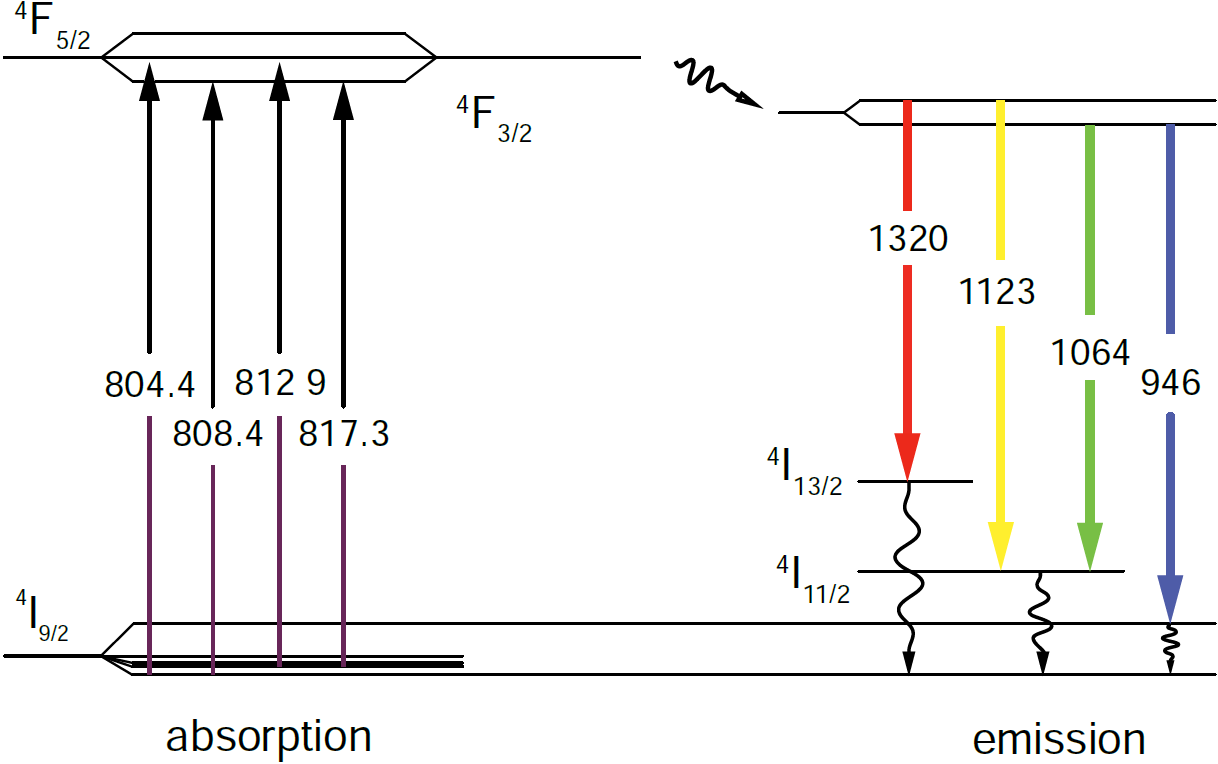
\includegraphics[width=\textwidth]{spectrum.png}
	\caption{Transitions in the Nd:YAG crystal \cite{lit:leybold}.}
	\label{fig:spectrum}
\end{figure}


\subsection{Nonlinear effect}
KTP crystal (Potassium titanyl phosphate, $\mathsf{K\,TiO\,PO_4}$)

two photon effect, quadratic

frequency doubling

energy conservation: $E = h \nu$
\begin{equation}
	\nu_2 = 2 \nu_1
\end{equation}

momentum conservation: $\vec p = \hbar \vec k$
\begin{equation}
	\vec k_2 = 2 \vec k_1
\end{equation}

$k = \frac{2 \pi}{\lambda}$
dispersion relation: $c = n c_0 = \lambda \nu$
\begin{equation}
2 = \frac{k_2}{k_1} = \frac{n_2 \nu_2}{n_1 \nu_1} = 2\;\frac{n_2}{n_1}
\end{equation}

Thus the refraction index of the material has to be the same for both wavelengths. As most materials show normal diffraction, i.e. $n(\lambda) \searrow$, 





% merge into literature:

% R. Willingale: \emph{lecture notes, Lasers and Quantum Optics}. University of Leicester 2007.\\
% \url{http://www.star.le.ac.uk/~zrw/courses/lect4313.html}
% crop image:
% http://www.star.le.ac.uk/~zrw/courses/lect4313_fig16.jpg

% http://www.atlas.uni-wuppertal.de/FP/anleitungen/fpI-09/diodenlaser.pdf
